\chapter{Wat planten nodig hebben}\label{ch:g4:what-plants-need}

Twee bakjes tuinkers staan op dezelfde vensterbank, op dezelfde dag
gezaaid. Het ene krijgt water, het andere niet --- en binnen een week
staat het verschil in het groen en het geel geschreven. Met bakjes,
\omterm{prop:g3:flowers-fruits-seeds:transform}{zaden} en geduld kun je \omterm{def:g1:plants-around-us:plant}{planten} zelf de vraag van dit hoofdstuk laten
beantwoorden: wat heeft een \omterm{def:g1:plants-around-us:plant}{plant} precies nodig om te leven en te groeien?

\section{Planten vragen stellen: de eerlijke proef}

\begin{method}[De eerlijke proef]\label{met:g4:what-plants-need:fairtest}
Om uit te zoeken of een \omterm{def:g1:plants-around-us:plant}{plant} iets nodig heeft --- water, licht, aarde,
warmte:
\begin{enumerate}
  \item neem \emph{twee} bakjes met dezelfde \omterm{def:g1:plants-around-us:plant}{planten}, op dezelfde
        manier gezaaid;
  \item behandel ze in alles precies gelijk \emph{behalve in het ene
        ding dat je onderzoekt} --- het ene krijgt het, het andere niet;
  \item wacht dagen of weken, en vergelijk;
  \item elk verschil moet van het ene ding komen dat je veranderd hebt:
        de proef was eerlijk.
\end{enumerate}
Het onaangeroerde bakje heet de \emph{controle}\index{controle
(proef)}: het laat zien wat er gebeurt als er niets ontbreekt.
\end{method}

\begin{example}[Waarom twee bakjes en niet één]\label{ex:g4:what-plants-need:control}
Stel dat één bakje zonder water verwelkt. Kwam dat door het ontbrekende
water --- of door een koude nacht, of door slechte zaadjes? Met een
begoten tweelingbakje dat er groen naast staat, gezaaid uit hetzelfde
zakje in dezelfde kamer, verdwijnt de twijfel: de tweelingen
verschilden alleen in water. Proeven met één bakje overtuigen niemand,
en een bioloog al helemaal niet.
\end{example}


\begin{omfigure}
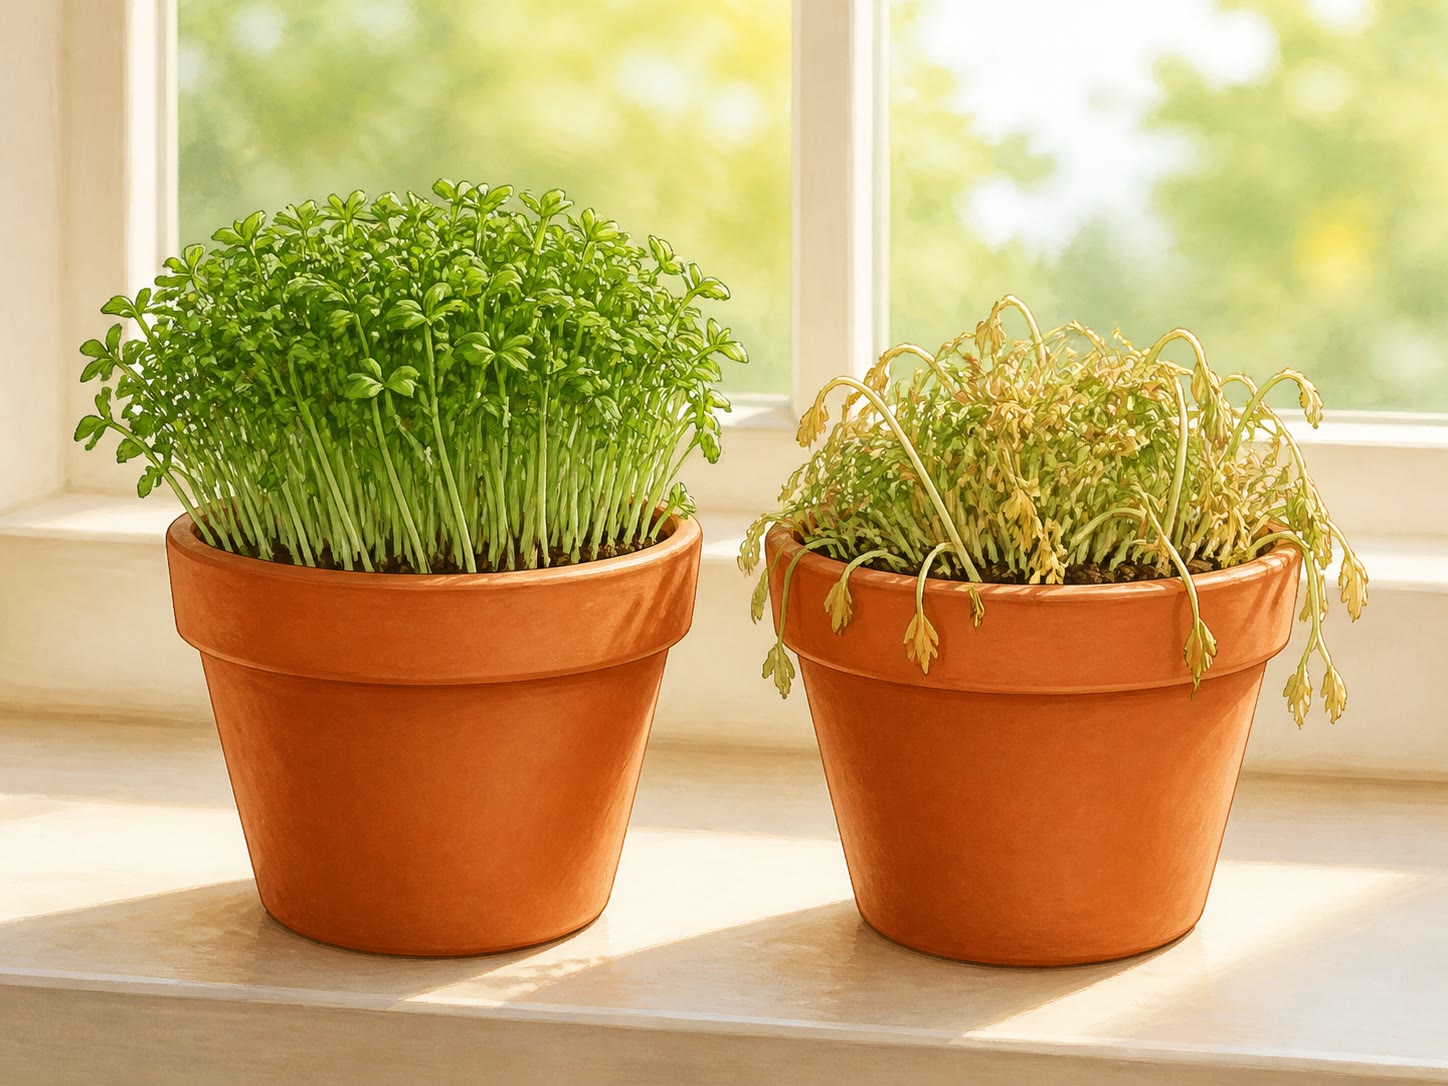
\includegraphics[width=0.58\linewidth]{images/book1/ai/g4-plants-cresspots.jpg}

{\small Dezelfde proef op een echte vensterbank, een week later: de
tweelingen verschillen nu in alles wat je ziet --- omdat ze in één ding
verschilden.}
\end{omfigure}

\section{Wat de proeven laten zien}

\begin{proposition}[De behoeften van een plant]\label{prop:g4:what-plants-need:needs}
Eerlijke proeven, voor elke behoefte op haar beurt uitgevoerd, laten
zien dat een \omterm{def:g1:plants-around-us:plant}{plant} nodig heeft:
\begin{itemize}
  \item \emph{water} --- het bakje zonder water verwelkt en gaat dood;
  \item \emph{licht} --- het bakje in de kast wordt bleek, lang en slap
        en geeft het dan op: geen licht, geen plantenvoedsel gemaakt;
  \item \emph{lucht} --- afgesloten van verse lucht stopt de groei;
  \item \emph{warmte} --- in de kou wachten \omterm{prop:g3:flowers-fruits-seeds:transform}{zaden}
        (\cref{prop:g2:from-seed-to-plant:needs}) en bevriest de groei
        tot stilstand;
  \item \emph{minerale zouten}\index{minerale zouten}: piepkleine
        hoeveelheden voedende stoffen die de \omterm{def:g1:plants-around-us:parts}{wortels} opgelost in het
        bodemwater opdrinken --- in zuiver water alleen komt een \omterm{def:g1:plants-around-us:plant}{plant}
        al snel tekort.
\end{itemize}
\end{proposition}
\admitted

\begin{example}[De bleke gevangene]\label{ex:g4:what-plants-need:pale}
De kastproef uit \cref{exo:g1:plants-around-us:8}, netjes gedaan met
een verlichte tweeling, geeft een opvallend resultaat: de gevangene is
niet alleen zielig maar \emph{bleekgeel} --- ze is gestopt met het
maken van haar groene stof --- en vreemd genoeg \emph{lang}, uitgerekt
alsof ze het ontbrekende licht zoekt. Groeien zonder licht is uitgeven
zonder te verdienen; als de reserves van het \omterm{def:g2:from-seed-to-plant:seed}{zaad} eenmaal op zijn,
stopt het.
\end{example}

\begin{remark}[Waarom tuinders de bodem voeden]\label{rem:g4:what-plants-need:soil}
Compost en mest zijn geen ``maaltijden'' voor de \omterm{def:g1:plants-around-us:plant}{plant} --- \omterm{def:g1:plants-around-us:plant}{planten} eten
niemand. Ze vullen de \omterm{prop:g4:what-plants-need:needs}{minerale zouten} van de bodem weer aan, die
oogsten jaar na jaar wegdragen. De compostbak uit
\cref{ex:g2:caring-for-nature:compost} sluit de kring: wat de bodem aan
de groenten gaf, geven de schillen aan de bodem terug.
\end{remark}

\section{Wat planten doen met wat ze opnemen}

\begin{proposition}[Planten maken hun eigen materie]\label{prop:g4:what-plants-need:make}
\omterm{def:g1:animals-around-us:animal}{Dieren} groeien door andere levende wezens te eten. Een \omterm{def:g1:plants-around-us:plant}{plant} eet
niemand: met water en \omterm{prop:g4:what-plants-need:needs}{minerale zouten} uit de bodem, met lucht en met de
\omterm{prop:g3:balanced-diet:jobs}{energie} van het \emph{licht} dat haar groene \omterm{def:g1:plants-around-us:parts}{bladeren} opvangen,
\emph{maakt ze haar eigen materie} --- nieuwe \omterm{def:g1:plants-around-us:parts}{stengels}, \omterm{def:g1:plants-around-us:parts}{bladeren},
\omterm{def:g1:plants-around-us:parts}{wortels} en \omterm{prop:g3:flowers-fruits-seeds:transform}{zaden}. Daarom is licht voor een \omterm{def:g1:plants-around-us:plant}{plant} net zo ernstig als eten
en drinken, en daarom keert het groene \omterm{def:g1:plants-around-us:parts}{blad} zich naar de hemel.
\end{proposition}
\admitted

\begin{example}[Een boom uit bijna niets]\label{ex:g4:what-plants-need:tree}
\omterm{def:g1:plants-around-us:plant}{Plant} een pit in een grote pot afgewogen aarde, wacht jaren, en er
staat een boompje --- en toch is de aarde bijna niets van haar gewicht
kwijt. Het hout van de boom is niet uit de pot geschept: het is
\emph{gemaakt}, uit water, lucht en licht, in de groene werkplaatsen
van de \omterm{def:g1:plants-around-us:parts}{bladeren}. Waar de materie van levende wezens vandaan komt, zal
ons in latere jaren opnieuw bezighouden.
\end{example}

\begin{remark}[Het groen verdient de kost voor iedereen]\label{rem:g4:what-plants-need:everyone}
Denk aan \cref{prop:g3:food-chains:start}: elke \omterm{def:g3:food-chains:chain}{voedselketen} begint met
een \omterm{def:g1:plants-around-us:plant}{plant}. Nu zien we waarom dat wel zo moet zijn --- \omterm{def:g1:plants-around-us:plant}{planten} zijn de
enige schakel die nieuwe materie uit niet-levende ingrediënten maakt.
Elke hap die iemand ergens eet, is eerst in een \omterm{def:g1:plants-around-us:parts}{blad} gemaakt.
\end{remark}

\section{Oefeningen}

\begin{exercise}[$\star$]\label{exo:g4:what-plants-need:1}
Noem de vijf behoeften van een \omterm{def:g1:plants-around-us:plant}{plant}.
\end{exercise}

\begin{exercise}[$\star$]\label{exo:g4:what-plants-need:2}
Hoeveel dingen mogen er in een eerlijke proef tussen de twee bakjes
verschillen? Hoe heet het onaangeroerde bakje?
\end{exercise}

\begin{exercise}[$\star$]\label{exo:g4:what-plants-need:3}
Beschrijf hoe een \omterm{def:g1:plants-around-us:plant}{plant} eruitziet die veertien dagen in het donker
heeft gestaan. Welke behoefte ontbrak, en wat kon ze niet maken?
\end{exercise}

\begin{exercise}[$\star$]\label{exo:g4:what-plants-need:4}
Wat zijn \omterm{prop:g4:what-plants-need:needs}{minerale zouten}, en hoe neemt de \omterm{def:g1:plants-around-us:plant}{plant} ze op?
\end{exercise}

\begin{exercise}[$\star$]\label{exo:g4:what-plants-need:5}
Waarom strooien tuinders compost, als \omterm{def:g1:plants-around-us:plant}{planten} niet eten?
\end{exercise}

\begin{exercise}[$\star$]\label{exo:g4:what-plants-need:6}
Hoe verschilt de manier van groeien van een \omterm{def:g1:plants-around-us:plant}{plant} van die van een \omterm{def:g1:animals-around-us:animal}{dier},
volgens \cref{prop:g4:what-plants-need:make}?
\end{exercise}

\begin{exercise}[$\star$]\label{exo:g4:what-plants-need:7}
In \cref{ex:g4:what-plants-need:tree} verloor de aarde in de pot
nauwelijks gewicht terwijl de boom groeide. Waar kwam de materie van de
boom vandaan?
\end{exercise}

\begin{exercise}[$\star$]\label{exo:g4:what-plants-need:8}
Probeer het: bedenk en doe de eerlijke waterproef uit de figuur met
tuinkers --- twee bakjes, één verschil. Noteer wat je na een week ziet.
\end{exercise}

\begin{exercise}[$\star\star$]\label{exo:g4:what-plants-need:9}
Lucas ``bewijst'' dat \omterm{def:g1:plants-around-us:plant}{planten} muziek nodig hebben: hij zong een maand
lang tegen één bakje, en dat bakje deed het prima. Wat ontbreekt er aan
zijn proef, volgens \cref{met:g4:what-plants-need:fairtest}? Bedenk de
versie die het werkelijk zou onderzoeken.
\end{exercise}

\begin{exercise}[$\star\star$]\label{exo:g4:what-plants-need:10}
Een waterplant groeit volledig onder water, zonder \omterm{def:g1:plants-around-us:parts}{wortels}, en toch
gezond. Aan welke van de vijf behoeften voldoet ze duidelijk nog steeds,
en hoe --- en welke behoefte levert haar water in plaats van de bodem?
\end{exercise}

\begin{exercise}[$\star\star\star$]\label{exo:g4:what-plants-need:11}
Twee identieke potten munt: de ene in zand met zuiver regenwater, de
andere in tuinaarde, allebei gelijk begoten en belicht. Na twee maanden
is de zandpot klein en geelachtig. Welke behoefte isoleert deze
eerlijke proef --- en waarom groeide de zandplant in het begin toch?
\end{exercise}
